\documentclass{article}

\usepackage[margin=1in]{geometry}
\usepackage{graphicx} % Allow image/pdf includes
\usepackage{extramarks} % Extra header marks (continued on next page)
\usepackage{amsmath} % Math enhancements
\usepackage{amsthm} % Theorem typesetting
\usepackage{amssymb} % Extended symbol collection
\usepackage{tikz} % Graphical element creation
\usetikzlibrary{automata,positioning}
\usepackage{algpseudocode} % Algorithm layout
\usepackage{enumitem} % Enumerate (lists)
\usepackage{ragged2e} % Alternative alignment
\usepackage{gensymb} % Generic symbols (degree, etc)
\usepackage{empheq} % Allow \boxed around \begin{empheq}
\usepackage{color,soul} % Highlighting
\usepackage{booktabs} % Enhanced table creation
\usepackage{multirow} % Table multi row
\usepackage{mathtools} % Math enhancements
\usepackage{bm} % Bold math
\usepackage[mathscr]{euscript} % Script variables
\usepackage{cancel} % Cancel through text
\usepackage{color,soul} % Highlighting
\usepackage{mathtools}
\usepackage{multirow}
\usepackage{mathrsfs}
\usepackage{physics}
\usepackage{gensymb}
\usepackage{siunitx}
\usepackage{subcaption}
\usepackage[]{algorithm2e}
\usepackage{float}
\usepackage[cache=false]{minted}
\renewcommand{\MintedPygmentize}{/Users/logan/miniconda/bin/pygmentize}
\usepackage[scaled]{beramono}
\usepackage[T1]{fontenc}
\usepackage{diagbox}

\setlength\parindent{0pt} % No indents
\setlength{\parskip}{1em} % Paragraph skip

\newcommand{\vx}{\mathbf{x}} % x vector
\newcommand{\vy}{\mathbf{y}} % x vector

\newcommand{\pageTitle}{MEEN 644 - Homework 4}
\newcommand{\pageAuthor}{Logan Harbour}

\begin{document}

\title{\LARGE \textbf{\pageTitle} \vspace{-0.3cm}}
\author{\large \pageAuthor}
\date{\vspace{-0.6cm} \large \today \vspace{-0.4cm}}

\maketitle

\section{Problem statement}

A viscous fluid (water at 20$^\circ$C: $\rho = 998.3$ kg/m$^3$ and $\mu = 1.002\times 10^{-3}$ N$\cdot$s/m$^2$) is trapped in a square 2-D cavity of dimension 0.2 m by 0.2 m. Either top or bottom walls are pulled to the right at a uniform velocity on purpose.

\begin{center}
	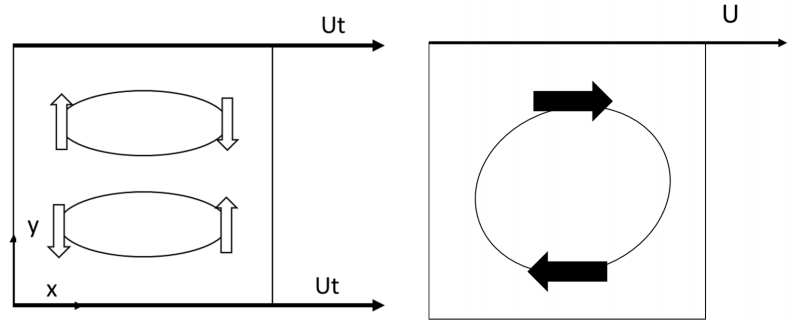
\includegraphics[width=0.6\linewidth]{statement}
	
	{\small Left: flow for problem (a) to verify symmetry; right: flow for problem (b) to compare with Roy et al. (2015).}
\end{center}

Write a finite-volume base computer program to predict the 2-D steady laminar flow field for Re = 400. Solve the velocity and pressure fields by linking them through the SIMPLE algorithm in a staggered grid. Represent the solution to the one-dimensional convection-diffusion problem using the power law scheme.

\begin{enumerate}[label=(\alph*)]
	\item \textbf{(60 points)} In order to verify your code for symmetry, make calculations using 5 x 5 uniformly sized control volumes (CVs). Declare convergence when $R_u$ and $R_v < 10^{-6}$ and $R_p < 10^{-5}$. Print your velocity and pressure fields up to 5 decimal places. 
	\item With the top plate pulled right at a constant velocity at Re = 400, calculate velocity and pressure fields using 8 x 8, 16 x 16, 32 x 32, 64 x 64, and 128 x 128 CVs.
	\begin{enumerate}[label=\roman*)]
		\item \textbf{(20 points)} Plot the centerline $u$ and $v$ velocities for each case (for centerline $u$ plot at $x = 0.1$ m, while for centerline $v$ plot at $y = 0.1$ m).
		\item \textbf{(20 points)} Compare your solutions of the 128 x 128 CV case with the benchmark solution of Roy et al (2015) on Tables 4 and 5.
	\end{enumerate}
\end{enumerate}

\section{Preliminaries}

\subsection{Two-dimensional diffusion-convection}

With two-dimensional diffusion and convection with constant material properties, we have the PDE
\begin{equation}
	\begin{cases}
		\pdv{u}{x} + \pdv{v}{y} = 0\,,\\
		\rho u \pdv{u}{x} + \rho v \pdv{v}{x} = - \pdv{P}{x} + \mu \pdv{^2u}{x^2} + \mu \pdv{^2u}{y^2}\,,\\
		\rho u \pdv{u}{y} + \rho v \pdv{v}{y} = - \pdv{P}{y} + \mu \pdv{^2v}{x^2} + \mu \pdv{^2v}{y^2}\,.
	\end{cases}
\end{equation}
where Dirichlet boundary conditions are applied on the boundary for $u$ and $v$.

The boundary conditions for problem (a) are:
\begin{equation}
	\begin{cases}
		u(x, L_y) = \frac{\mu \text{Re}}{\rho L_x}\,, \\
		u(L_x, y) = 0 \,, \\
		u(x, 0) = \frac{\mu \text{Re}}{\rho L_x} \,, \\
		u(0, y) = 0 \,, \\
		v(x, L_y) = 0\,, \\
		v(L_x, y) = 0 \,, \\
		v(x, 0) = 0\,, \\
		v(0, y) = 0 \,,
	\end{cases}\,,
\end{equation}
and the boundary conditions for problem (b) are:
\begin{equation}
	\begin{cases}
		u(x, L_y) = \frac{\mu \text{Re}}{\rho L_x}\,, \\
		u(L_x, y) = 0 \,, \\
		u(x, 0) = 0 \,, \\
		u(0, y) = 0 \,, \\
		v(x, L_y) = 0\,, \\
		v(L_x, y) = 0 \,, \\
		v(x, 0) = 0\,, \\
		v(0, y) = 0 \,.
	\end{cases}\,.
\end{equation}

\subsection{Solving methodology}

Using the SIMPLE algorithm, the problem is solved in the following order:
\begin{enumerate}
	\item Explicitly fill the boundary conditions into the $u$ and $v$ solution vector in order to enforce them in all of the integrations that follow.
	\item Guess a pressure field, $p^*$.
	\item Use the guessed (or previously iterated) pressure field to obtain the velocity guesses, $u^*$ and $v^*$, as discussed in \ref{subsec:velocity-guess}.
	\item Solve the pressure correction, $p'$, as discussed in \ref{subsec:pc-solve}.
	\item Compute the velocity corrections, $u'$ and $v'$, and correct the velocity and pressure field, as discussed in \ref{subsec:correction}.
	\item Check for convergence. If not converged, return to 2.
\end{enumerate}

\subsection{Domain discretization}

The domain of size $L_x \times L_y$ is discretized into $N_x \times N_y$ uniformly sized control volumes with $\Delta x = L_x / N_x$ and $\Delta y = L_y / N_y$. The numbering for all variables begins at the origin at $(i, j) = (0, 0)$. The maximum index for each variable, $\phi$, is defined as $(M_x^\phi, M_y^\phi)$.

\begin{figure}[H]
	\centering
	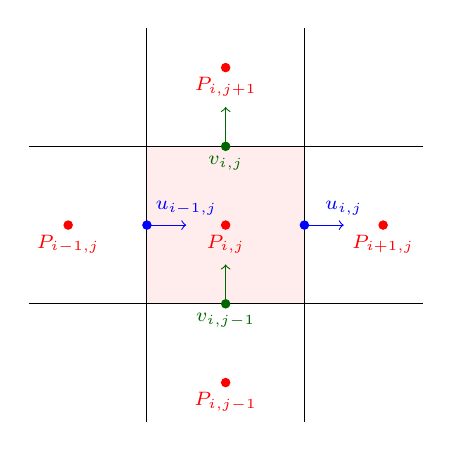
\begin{tikzpicture}[scale=1, style={font=\scriptsize}]
		\tikzset{dimen/.style={<->,>=latex,thin,every rectangle node/.style={fill=white,midway,font=\small}}}
		
		\filldraw[red!7] (0,0) -- (2,0) -- (2,2) -- (0, 2) -- cycle;
		\draw (-1.5, 0) -- (3.5, 0);
		\draw (-1.5, 2) -- (3.5, 2);
		\draw (0, -1.5) -- (0, 3.5);
		\draw (2, -1.5) -- (2, 3.5);
		
		\filldraw[red] (1, 1) circle (1.5pt);
		\filldraw[blue] (0, 1) circle (1.5pt);
		\filldraw[green!40!black] (1, 0) circle (1.5pt);
		\filldraw[blue] (2, 1) circle (1.5pt);
		\filldraw[green!40!black] (1, 2) circle (1.5pt);
		\filldraw[red] (-1, 1) circle (1.5pt);
		\filldraw[red] (3, 1) circle (1.5pt);
		\filldraw[red] (1, 3) circle (1.5pt);
		\filldraw[red] (1, -1) circle (1.5pt);
		
		\draw [->,blue] (0, 1) -- (0.5, 1);
		\draw [->,blue] (2, 1) -- (2.5, 1);
		\draw [->,green!40!black] (1, 0) -- (1,0.5);
		\draw [->,green!40!black] (1, 2) -- (1,2.5);
		
		\node[below, red] at (1, 1) {$P_{i, j}$};
		\node[below, red] at (3, 1) {$P_{i+1, j}$};
		\node[below, red] at (-1, 1) {$P_{i-1, j}$};
		\node[below, red] at (1, 3) {$P_{i, j+1}$};
		\node[below, red] at (1, -1) {$P_{i, j-1}$};
		
		\node[above,blue] at (0.5, 1) {$u_{i-1,j}$};
		\node[above,blue] at (2.5, 1) {$u_{i,j}$};
		\node[below,green!40!black] at (1, 0) {$v_{i,j-1}$};
		\node[below,green!40!black] at (1, 2) {$v_{i,j}$};
	\end{tikzpicture}
	\caption{An internal pressure control volume.}
	\label{fig:CV-p}
\end{figure}

\begin{figure}[H]
	\centering
	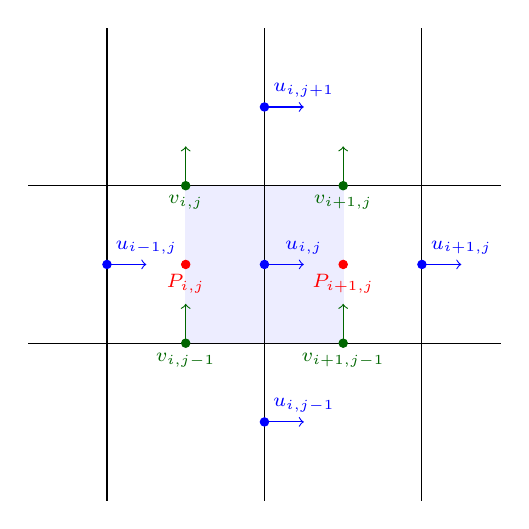
\begin{tikzpicture}[scale=1, style={font=\scriptsize}]
		\tikzset{dimen/.style={<->,>=latex,thin,every rectangle node/.style={fill=white,midway,font=\small}}}
		
		\filldraw[blue!7] (1,0) -- (3,0) -- (3,2) -- (1, 2) -- cycle;
		\draw (-1, 0) -- (5, 0);
		\draw (-1, 2) -- (5, 2);
		\draw (0, -2) -- (0, 4);
		\draw (2, -2) -- (2, 4);
		\draw (4, -2) -- (4, 4);
		
		\filldraw[red] (1, 1) circle (1.5pt);
		\filldraw[red] (3, 1) circle (1.5pt);
		\filldraw[green!40!black] (1, 2) circle (1.5pt);
		\filldraw[green!40!black] (1, 0) circle (1.5pt);
		\filldraw[green!40!black] (3, 0) circle (1.5pt);
		\filldraw[green!40!black] (3, 2) circle (1.5pt);
		\filldraw[blue] (2, 1) circle (1.5pt);
		\filldraw[blue] (4, 1) circle (1.5pt);
		\filldraw[blue] (0, 1) circle (1.5pt);
		\filldraw[blue] (2, 3) circle (1.5pt);
		\filldraw[blue] (2, -1) circle (1.5pt);
		
		\draw [->,blue] (0, 1) -- (0.5, 1);
		\draw [->,blue] (2, 1) -- (2.5, 1);
		\draw [->,blue] (4, 1) -- (4.5, 1);
		\draw [->,blue] (2, 3) -- (2.5, 3);
		\draw [->,blue] (2, -1) -- (2.5, -1);
		\draw [->,green!40!black] (1, 0) -- (1,0.5);
		\draw [->,green!40!black] (1, 2) -- (1,2.5);
		\draw [->,green!40!black] (3, 0) -- (3,0.5);
		\draw [->,green!40!black] (3, 2) -- (3,2.5);
		
		\node[below, red] at (1, 1) {$P_{i, j}$};
		\node[below, red] at (3, 1) {$P_{i+1, j}$};
		
		\node[above,blue] at (0.5, 1) {$u_{i-1,j}$};
		\node[above,blue] at (2.5, 1) {$u_{i,j}$};
		\node[above,blue] at (4.5, 1) {$u_{i+1,j}$};
		\node[above,blue] at (2.5, 3) {$u_{i,j+1}$};
		\node[above,blue] at (2.5, -1) {$u_{i,j-1}$};
		\node[below,green!40!black] at (1, 0) {$v_{i,j-1}$};
		\node[below,green!40!black] at (1, 2) {$v_{i,j}$};
		\node[below,green!40!black] at (3, 0) {$v_{i+1,j-1}$};
		\node[below,green!40!black] at (3, 2) {$v_{i+1,j}$};
	\end{tikzpicture}
	\caption{An internal $u$-velocity control volume.}
	\label{fig:CV-u}
\end{figure}

\begin{figure}[H]
	\centering
	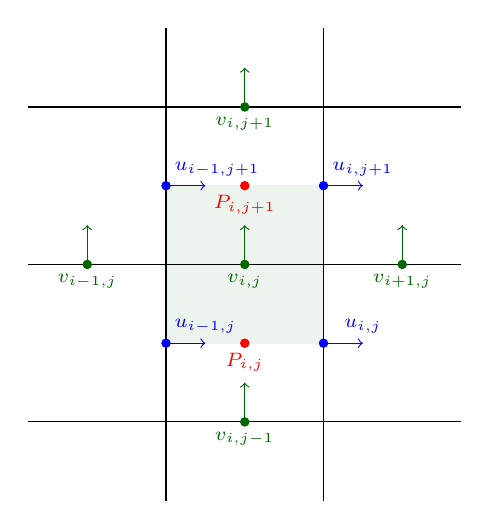
\begin{tikzpicture}[scale=1, style={font=\scriptsize}]
		\tikzset{dimen/.style={<->,>=latex,thin,every rectangle node/.style={fill=white,midway,font=\small}}}
		
		\filldraw[green!40!black!7] (0,1) -- (2,1) -- (2,3) -- (0, 3) -- cycle;
		\draw (-1.75, 0) -- (3.75, 0);
		\draw (-1.75, 2) -- (3.75, 2);
		\draw (-1.75, 4) -- (3.75, 4);
		\draw (0, -1) -- (0, 5);
		\draw (2, -1) -- (2, 5);
		
		\filldraw[red] (1, 1) circle (1.5pt);
		\filldraw[red] (1, 3) circle (1.5pt);
		\filldraw[blue] (0, 1) circle (1.5pt);
		\filldraw[blue] (2, 1) circle (1.5pt);
		\filldraw[blue] (0, 3) circle (1.5pt);
		\filldraw[blue] (2, 3) circle (1.5pt);
		\filldraw[green!40!black] (1, 0) circle (1.5pt);
		\filldraw[green!40!black] (1, 2) circle (1.5pt);
		\filldraw[green!40!black] (1, 4) circle (1.5pt);
		\filldraw[green!40!black] (-1, 2) circle (1.5pt);
		\filldraw[green!40!black] (3, 2) circle (1.5pt);
		
		\draw [->,blue] (0, 1) -- (0.5, 1);
		\draw [->,blue] (2, 1) -- (2.5, 1);
		\draw [->,blue] (0, 3) -- (0.5, 3);
		\draw [->,blue] (2, 3) -- (2.5, 3);
		\draw [->,green!40!black] (1, 0) -- (1,0.5);
		\draw [->,green!40!black] (1, 2) -- (1,2.5);
		\draw [->,green!40!black] (1, 4) -- (1, 4.5);
		\draw [->,green!40!black] (-1, 2) -- (-1, 2.5);
		\draw [->,green!40!black] (3, 2) -- (3, 2.5);
		
		\node[below, red] at (1, 1) {$P_{i, j}$};
		\node[below, red] at (1, 3) {$P_{i, j+1}$};
		\node[above,blue] at (0.5, 1) {$u_{i-1,j}$};
		\node[above,blue] at (2.5, 1) {$u_{i,j}$};
		\node[above,blue] at (0.65, 3) {$u_{i-1,j+1}$};
		\node[above,blue] at (2.5, 3) {$u_{i,j+1}$};
		\node[below,green!40!black] at (1, 2) {$v_{i,j}$};
		\node[below,green!40!black] at (1, 0) {$v_{i,j-1}$};
		\node[below,green!40!black] at (1, 4) {$v_{i,j+1}$};
		\node[below,green!40!black] at (-1, 2) {$v_{i-1,j}$};
		\node[below,green!40!black] at (3, 2) {$v_{i+1,j}$};
	\end{tikzpicture}
	\caption{An internal $v$-velocity control volume.}
	\label{fig:CV-v}
\end{figure}

\subsection{Velocity guess}
\label{subsec:velocity-guess}

Define the Pechlet number on each boundary of a CV for variable $\phi$ centered at node $\phi_{i,j}$ as
\begin{equation}
	P^{\phi_{i,j}}_\text{bd} = \frac{F^{\phi_{i,j}}_\text{bd}}{D^{\phi_{i,j}}_\text{bd}} \,, \quad \text{where} \quad \text{bd} = [n, e, s, w] \quad \text{and} \quad \phi = [u, v]\,.
\end{equation}

The integration of the $x$ and $y$-momentum equations (generalizing again with $\phi = [u, v]$) using the power-law scheme results in the equation (for $i = 1, \ldots, M_x^\phi - 1\,\,,\, j = 1, \ldots, M_y^\phi - 1$)
\begin{subequations}
	\label{eq:power}
	\begin{align}
		a^{\phi_{i,j}}_p \phi^*_{i,j} & = a^{\phi_{i,j}}_n \phi^*_{i, j+1} + a^{\phi_{i,j}}_e \phi^*_{i+1, j} + a^{\phi_{i,j}}_s \phi^*_{i, j-1} + a^{\phi_{i,j}}_w \phi^*_{i-1, j} + a_b^{\phi_{i,j}}\,,\\
		a^{\phi_{i,j}}_n & = D^{\phi_{i,j}}_n \max \left[0, (1 - 0.1 |P^{\phi_{i,j}}_n|)^5\right] + \max \left[ -F^{\phi_{i,j}}_n, 0 \right]\,, \\
		a^{\phi_{i,j}}_e & = D^{\phi_{i,j}}_e \max \left[0, (1 - 0.1 |P^{\phi_{i,j}}_e|)^5\right] + \max \left[ -F^{\phi_{i,j}}_e, 0 \right]\,, \\
		a^{\phi_{i,j}}_s & = D^{\phi_{i,j}}_s \max \left[0, (1 - 0.1 |P^{\phi_{i,j}}_s|)^5\right] + \max \left[ F^{\phi_{i,j}}_s, 0 \right]\,, \\
		a^{\phi_{i,j}}_w & = D^{\phi_{i,j}}_w \max \left[0, (1 - 0.1 |P^{\phi_{i,j}}_w|)^5\right] + \max \left[ F^{\phi_{i,j}}_w, 0 \right]\,, \\
		a^{\phi_{i,j}}_p & = a^{\phi_{i,j}}_n + a^{\phi_{i,j}}_e + a^{\phi_{i,j}}_s + a^{\phi_{i,j}}_w\,, \\
		a^{\phi_{i,j}}_b & = \begin{cases}
			\Delta y (p^*_{i,j} - p^*_{i+1,j})\,, & \phi = u\\
			\Delta x (p^*_{i,j} - p^*_{i, j+1})\,, & \phi = v
		\end{cases}\,.
	\end{align}
\end{subequations}

\subsubsection{$u$-velocity guess update}

In all discussion that follow, we are considering a $u$-CV defined by the central node $u_{i,j}$. For simplicity we will define the width of each $u$-CV as
\begin{equation}
	\Delta x^{u_{i,j}} = \begin{cases}
		\Delta x\,, & 1 < i < M_x^u - 1 \\
		\frac{3}{2} \Delta x\,, & \text{otherwise}
	\end{cases}\,,
\end{equation}
and we will also define the $y$-distance from $u_{i,j}$ to the north and south pressure interfaces, respectively, as
\begin{subequations}
	\begin{align}
		\delta y^{u_{i,j}}_{p_n} & = \begin{cases}
		\frac{1}{2} \Delta y\,, & j = M_y^u - 1\,, \\
		\Delta y\,, & \text{otherwise}
		\end{cases}\,, \\
		\delta y^{u_{i,j}}_{p_s} & = \begin{cases}
		\frac{1}{2} \Delta y\,, & j = 1\,, \\
		\Delta y\,, & \text{otherwise}
		\end{cases}\,.
	\end{align}
\end{subequations}
The diffusion coefficients are then defined as
\begin{subequations}
	\begin{align}
		D_n^{u_{i,j}} & = \frac{\mu \Delta x^{u_{i,j}}}{\delta y^{u_{i,j}}_{p_n}}\,,\\
		D_e^{u_{i,j}} & = \frac{\mu\Delta y}{\Delta x}\,,\\
		D_s^{u_{i,j}} & = \frac{\mu \Delta x^{u_{i,j}}}{\delta y^{u_{i,j}}_{p_s}}\,,\\
		D_w^{u_{i,j}} & = \frac{\mu\Delta y}{\Delta x}\,.
	\end{align}
\end{subequations}
Lastly, the flow rates are defined as
\begin{subequations}
	\begin{align}
		F_n^{u_{i,j}} & = \rho \Delta x^{u_{i,j}} \begin{cases}
			\frac{1}{6} \left(v^*_{0, j} + 3 v^*_{1, j} + 2 v^*_{2, j} \right)\,, & i = 1 \\
			\frac{1}{6} \left(2 v^*_{i, j} + 3 v^*_{i + 1, j} + v^*_{i + 2, j} \right)\,, & i = M_x^u - 1 \\
			\frac{1}{2} \left(v^*_{i, j} + v^*_{i + 1, j}\right)\,, & \text{otherwise} 
		\end{cases}\,, \\
		F_e^{u_{i,j}} & = \rho \Delta y \begin{cases}
			u^*_{M_x^u, j}\,, & i = M_x^u - 1 \\
			\frac{1}{2} \left(u^*_{i+1, j} + u^*_{i,j}\right)\,, & \text{otherwise}
		\end{cases}\,, \\
		F_s^{u_{i,j}} & = \rho \Delta x^{u_{i,j}} \begin{cases}
			\frac{1}{6} \left(v^*_{0, j - 1} + 3 v^*_{1, j - 1} + 2 v^*_{2, j - 1} \right)\,, & i = 1 \\
			\frac{1}{6} \left(2 v^*_{i, j - 1} + 3 v^*_{i + 1, j - 1} + v^*_{i + 2, j - 1} \right)\,, & i = M_x^u - 1 \\
			\frac{1}{2} \left(v^*_{i, j - 1} + v^*_{i + 1, j - 1}\right)\,, & \text{otherwise} 
			\end{cases} \\
		F_w^{u_{i,j}} & = \rho \Delta y \begin{cases}
			u^*_{0, j}\,, & i = 1 \\
			\frac{1}{2} \left( u^*_{i - 1, j} + u^*_{i, j} \right)\,, & \text{otherwise}
		\end{cases}\,.
	\end{align}
\end{subequations}

\subsubsection{$v$-velocity guess update}

Similarly, we will consider a $v$-CV defined by the central node $v_{i,j}$. The width of each $v$-CV is defined as
\begin{equation}
	\Delta y^{v_{i,j}} = \begin{cases}
		\Delta y \,, & 1 < j < M_y^v - 1 \\
		\frac{3}{2} \Delta y \,, & \text{otherwise}
	\end{cases}\,,
\end{equation}
and we will also define the $x$-distance from $v_{i,j}$ to the east and west pressure interfaces, respectively, as
\begin{subequations}
	\begin{align}
		\delta x^{v_{i,j}}_{p_e} & = \begin{cases}
			\frac{1}{2} \Delta x\,, & i = M_x^v - 1 \\
			\Delta x \,, & \text{otherwise}
		\end{cases}\,, \\
		\delta x^{v_{i,j}}_{p_w} & = \begin{cases}
			\frac{1}{2} \Delta x\,, & i = 1\,, \\
			\Delta x\,, & \text{otherwise}
		\end{cases}\,.
	\end{align}
\end{subequations}
The diffusion coefficients are then defined as
\begin{subequations}
	\begin{align}
		D_n^{v_{i,j}} & = \frac{\mu \Delta x}{\Delta y}\,,\\
		D_e^{v_{i,j}} & = \frac{\mu \Delta y^{v_{i,j}}}{\delta x^{v_{i,j}}_{p_e}}\,,\\
		D_s^{v_{i,j}} & = \frac{\mu \Delta x}{\Delta y}\,,\\
		D_w^{v_{i,j}} & = \frac{\mu\Delta y^{v_{i,j}}}{\delta x^{v_{i,j}}_{p_w}}\,.
	\end{align}
\end{subequations}
Lastly, the flow rates are defined as
\begin{subequations}
	\begin{align}
		F_n^{v_{i,j}} & = \rho \Delta x \begin{cases}
			v^*_{i, M_y^v}\,, & j = M_y^v - 1 \\
			\frac{1}{2} \left(v^*_{i, j+1} + v^*_{i,j}\right)\,, & \text{otherwise}
		\end{cases}\,, \\
		F_e^{v_{i,j}} & = \rho \Delta y^{v_{i,j}} \begin{cases}
			\frac{1}{6} \left( u^*_{i, 0} + 3 u^*_{i, 1} + 2 u^*_{i, 2} \right)\,, & j = 1 \\
			\frac{1}{6} \left( 2 u^*_{i, j} + 3 u^*_{i, j + 1} + 2 u^*_{i, j + 2} \right)\,, & j = M_y^v - 1 \\
			\frac{1}{2} \left( u^*_{i, j} + u^*_{i, j + 1} \right)\,, & \text{otherwise} 
		\end{cases}\,, \\
		F_s^{v_{i,j}} & = \rho \Delta x \begin{cases}
			v^*_{i, 0}\,, & j = 1 \\
			\frac{1}{2} \left(v^*_{i, j+ 1} + v^*_{i,j}\right)\,, & \text{otherwise}
		\end{cases}\,, \\
		F_w^{v_{i,j}} & = \rho \Delta y^{v_{i,j}} \begin{cases}
			\frac{1}{6} \left( u^*_{i - 1, 0} + 3 u^*_{i - 1, 1} + 2 u^*_{i - 1, 2} \right)\,, & j = 1 \\
			\frac{1}{6} \left( 2 u^*_{i - 1, j} + 3 u^*_{i - 1, j + 1} + 2 u^*_{i - 1, j + 2} \right)\,, & j = M_y^v - 1 \\
			\frac{1}{2} \left( u^*_{i - 1, j} + u^*_{i - 1, j + 1} \right)\,, & \text{otherwise} 
			\end{cases}\,.
	\end{align}
\end{subequations}

\subsection{Pressure correction solve}
\label{subsec:pc-solve}

At convergence, $u' = v' = p' = 0$, therefore it is irrelevant as to how we find them. Subtracting (exact - guessed) forms of Equation \eqref{eq:power} one obtains
\begin{subequations}
	\begin{align}
		a^{u_{i,j}}_p u'_{i,j} & = a^{u_{i,j}}_n u'_{i, j+1} + a^{u_{i,j}}_e u'_{i+1, j} + a^{u_{i,j}}_s u'_{i, j-1} + a^{u_{i,j}}_w u'_{i-1, j} + \Delta y (p'_{i,j} - p'_{i+1,j}) \,, \\
		a^{v_{i,j}}_p v'_{i,j} & = a^{v_{i,j}}_n v'_{i, j+1} + a^{v_{i,j}}_e v'_{i+1, j} + a^{v_{i,j}}_s v'_{i, j-1} + a^{v_{i,j}}_w v'_{i-1, j} + \Delta x (p'_{i,j} - p'_{i, j+1}) \,.
	\end{align}
\end{subequations}
Drop the neighbor terms in the equations above (implying that velocity corrections are local) to obtain
\begin{subequations}
	\label{eq:velocity_corrector}
	\begin{align}
		u_{i,j}' & = \frac{\Delta y}{a_p^{u_{i,j}}} (p'_{i,j} - p'_{i+1,j})\,, \\
		v_{i,j}' & = \frac{\Delta x}{a_p^{v_{i,j}}} (p'_{i,j} - p'_{i, j+1})\,.
	\end{align}
\end{subequations}
Integrate the continuity equation over a $p$-CV defined by the central node $p_{i,j}$ and substitute $u = u^* + u'$, $v = v^* + v'$, and the above Equations to obtain
\begin{subequations}
	\label{eq:pc}
	\begin{align}
		a^{p'_{i,j}}_p p'_{i,j} & = a^{p'_{i,j}}_n p'_{i, j+1} + a^{p'_{i,j}}_e p'_{i+1, j} + a^{p'_{i,j}}_s p'_{i, j-1} + a^{p'_{i,j}}_w p'_{i-1, j} + a_b^{p'_{i,j}}\,,\\
		a^{p'_{i,j}}_n & = \begin{cases}
			\rho \Delta x^2 / a_p^{v_{i, j}}\,, & j < M_y^p - 1 \\
			0\,, & \text{otherwise}
		\end{cases}\,, \\
		a^{p'_{i,j}}_e & = \begin{cases}
			\rho \Delta y^2 / a_p^{u_{i, j}}\,, & i < M_x^p - 1 \\
			0\,, & \text{otherwise}
		\end{cases}\,, \\
		a^{p'_{i,j}}_s & = \begin{cases}
			\rho \Delta x^2 / a_p^{v_{i, j - 1}}\,, & j > 1 \\
			0\,, & \text{otherwise}
		\end{cases}\,, \\
		a^{p'_{i,j}}_w & = \begin{cases}
			\rho \Delta y^2 / a_p^{u_{i - 1, j}}\,, & i > 1 \\
			0\,, & \text{otherwise}
		\end{cases}\,, \\
		a^{p'_{i,j}}_p & = a^{p'_{i,j}}_n + a^{p'_{i,j}}_e + a^{p'_{i,j}}_s + a^{p'_{i,j}}_w\,, \\
		a^{p'_{i,j}}_b & = \rho \left(\Delta y (u_{i - 1, j}^* - u^*_{i,j}) + \Delta x(v^*_{i, j - 1} - v^*_{i,j})\right)\,.
	\end{align}
\end{subequations}

\subsection{Velocity and pressure correction}
\label{subsec:correction}

Lastly, the velocities are then updated using Equation \eqref{eq:velocity_corrector} with
\begin{subequations}
	\begin{align}
		u_{i,j} & = u_{i,j} + \frac{\Delta y}{a_p^{u_{i,j}}} (p'_{i,j} - p'_{i+1,j})\,,\quad i = 1, \ldots, M_x^u - 1\,, \quad j = 1, \ldots, M_y^u - 1\,, \\
		v_{i,j} & = v_{i,j} + \frac{\Delta x}{a_p^{v_{i,j}}} (p'_{i,j} - p'_{i, j+1})\,,\quad i = 1, \ldots, M_x^v - 1\,, \quad j = 1, \ldots, M_y^v - 1\,,
	\end{align}
\end{subequations}
and the pressures  (take note of the relaxation parameter $\alpha_p$) with
\begin{equation}
	p_{i,j} = p_{i,j} + \alpha_p p'_{i,j} \,,\quad i = 1, \ldots, M_x^p - 1\,, \quad j = 1, \ldots, M_y^p - 1\,.
\end{equation}

\subsection{System solver}

The systems in Equations  \eqref{eq:power} and \eqref{eq:pc} are solved using the line-by-line method with TDMA as the matrix solver. In this method, a tri-diagonal system is formed as the terms from one of the dimensions are lagged. Consider the simple system
\begin{equation}
	a_p^{i,j} \phi_{i,j} = a_n^{i,j} \phi_{i,j+1} + a_e^{i,j} \phi_{i+1,j} + a_s^{i,j} \phi_{i,j-1} + a_w^{i,j} \phi_{i-1,j} + a_b^{i,j}\,, \quad i = 1, \ldots, N_x\,, \quad j = 1, \ldots, N_y\,.
\end{equation}
Now, consider $\phi^*$ to be a \textit{lagged} value of $\phi$, i.e., it is known and is moved to the right hand side of each equation. In solving a single physical column $i$ using the line-by-line method, the following system is solved:
\begin{equation}
	a_p^{i,j} \phi_{i,j} = a_n^{i,j} \phi_{i,j+1} + a_e^{i,j} \phi^*_{i+1,j} + a_s^{i,j} \phi_{i,j-1} + a_w^{i,j} \phi^*_{i-1,j} + a_b^{i,j}\,, \quad \quad j = 1, \ldots, N_y\,.
\end{equation}
In solving a single physical row $j$ using the line-by-line method, the following system is solved:
\begin{equation}
	a_p^{i,j} \phi_{i,j} = a_n^{i,j} \phi^*_{i,j+1} + a_e^{i,j} \phi_{i+1,j} + a_s^{i,j} \phi^*_{i,j-1} + a_w^{i,j} \phi_{i-1,j} + a_b^{i,j}\,, \quad \quad i = 1, \ldots, N_x\,.
\end{equation}

\section{Results}

\subsection{Problem a: Lid driven cavity, symmetry check}

Symmetric solutions were identified for problem (a), as presented in Tables \ref{table:symmetric-u}, \ref{table:symmetric-v}, and \ref{table:symmetric-p} below.

\def\arraystretch{1.3}
\begin{table}[H]
	\scriptsize
	\centering
	\caption{The $u$-velocity solution with 5x5 pressure CVs and symmetric BCs.}
	\vspace{0.2cm}
	\sisetup{output-exponent-marker = \text{E}, table-format=2.5e1,group-digits=false,retain-zero-exponent=true}
	\begin{tabular}{c|S|S|S|S|S|S}
		& {1} & {2} & {3} & {4} & {5} & {6} \\
		\hline
		1 & +2.00741e-03 & +2.00741e-03 & +2.00741e-03 & +2.00741e-03 & +2.00741e-03 & +2.00741e-03 \\
		2 & +0.00000e+00 & +1.69059e-04 & +2.96268e-04 & +3.47982e-04 & +2.74870e-04 & +0.00000e+00 \\
		3 & +0.00000e+00 & -6.05705e-05 & -1.24904e-04 & -1.54163e-04 & -1.09384e-04 & +0.00000e+00 \\
		4 & +0.00000e+00 & -2.16978e-04 & -3.42727e-04 & -3.87638e-04 & -3.30974e-04 & +0.00000e+00 \\
		5 & +0.00000e+00 & -6.05705e-05 & -1.24904e-04 & -1.54163e-04 & -1.09384e-04 & +0.00000e+00 \\
		6 & +0.00000e+00 & +1.69059e-04 & +2.96268e-04 & +3.47982e-04 & +2.74870e-04 & +0.00000e+00 \\
		7 & +2.00741e-03 & +2.00741e-03 & +2.00741e-03 & +2.00741e-03 & +2.00741e-03 & +2.00741e-03
	\end{tabular}
	\label{table:symmetric-u}
\end{table}

\def\arraystretch{1.3}
\begin{table}[H]
	\scriptsize
	\centering
	\caption{The $v$-velocity solution with 5x5 pressure CVs and symmetric BCs.}
	\vspace{0.2cm}
	\sisetup{output-exponent-marker = \text{E}, table-format=2.5e1,group-digits=false,retain-zero-exponent=true}
	\begin{tabular}{c|S|S|S|S|S|S|S}
		& {1} & {2} & {3} & {4} & {5} & {6} & {7} \\
		\hline
		1 & +0.00000e+00 & +0.00000e+00 & +0.00000e+00 & +0.00000e+00 & +0.00000e+00 & +0.00000e+00 & +0.00000e+00 \\
		2 & +0.00000e+00 & -1.69059e-04 & -1.27208e-04 & -5.17144e-05 & +7.31116e-05 & +2.74870e-04 & +0.00000e+00 \\
		3 & +0.00000e+00 & -1.08489e-04 & -6.28747e-05 & -2.24555e-05 & +2.83322e-05 & +1.65487e-04 & +0.00000e+00 \\
		4 & +0.00000e+00 & +1.08489e-04 & +6.28746e-05 & +2.24555e-05 & -2.83322e-05 & -1.65487e-04 & +0.00000e+00 \\
		5 & +0.00000e+00 & +1.69059e-04 & +1.27208e-04 & +5.17144e-05 & -7.31116e-05 & -2.74870e-04 & +0.00000e+00 \\
		6 & +0.00000e+00 & +0.00000e+00 & +0.00000e+00 & +0.00000e+00 & +0.00000e+00 & +0.00000e+00 & +0.00000e+00
	\end{tabular}
	\label{table:symmetric-v}
\end{table}

\def\arraystretch{1.3}
\begin{table}[H]
	\scriptsize
	\centering
	\caption{The $p$ solution with 5x5 pressure CVs and symmetric BCs.}
	\vspace{0.2cm}
	\sisetup{output-exponent-marker = \text{E}, table-format=2.5e1,group-digits=false,retain-zero-exponent=true}
	\begin{tabular}{c|S|S|S|S|S|S|S}
		& {1} & {2} & {3} & {4} & {5} & {6} & {7} \\
		\hline
		1 & -9.59831e-05 & -9.59831e-05 & -5.96700e-06 & +1.14365e-05 & +6.78274e-05 & +2.13791e-04 & +2.13791e-04 \\
		2 & -9.59831e-05 & -9.59831e-05 & -5.96700e-06 & +1.14365e-05 & +6.78274e-05 & +2.13791e-04 & +2.13791e-04 \\
		3 & +1.42128e-06 & +1.42128e-06 & -2.15270e-05 & -3.57174e-05 & -1.98216e-05 & +7.52326e-05 & +7.52326e-05 \\
		4 & +1.86045e-05 & +1.86045e-05 & -9.11188e-06 & -2.11868e-05 & +1.15363e-05 & +8.26938e-05 & +8.26938e-05 \\
		5 & +1.42128e-06 & +1.42128e-06 & -2.15270e-05 & -3.57174e-05 & -1.98216e-05 & +7.52326e-05 & +7.52326e-05 \\
		6 & -9.59831e-05 & -9.59831e-05 & -5.96700e-06 & +1.14365e-05 & +6.78274e-05 & +2.13791e-04 & +2.13791e-04 \\
		7 & -9.59831e-05 & -9.59831e-05 & -5.96700e-06 & +1.14365e-05 & +6.78274e-05 & +2.13791e-04 & +2.13791e-04
	\end{tabular}
	\label{table:symmetric-p}
\end{table}

\subsection{Problem b: Lid driven cavity, top right BC}

The requirements for problem (b) part i and ii were combined into Figure \ref{fig:p2} as seen below. With increasing grid refinement, both centerline velocity profiles approached towards the reference solution obtained from Roy et. al. In addition, a once-more-refined run is compared with 256x256 CVs with good agreement.

\begin{figure}[H]
	\centering
	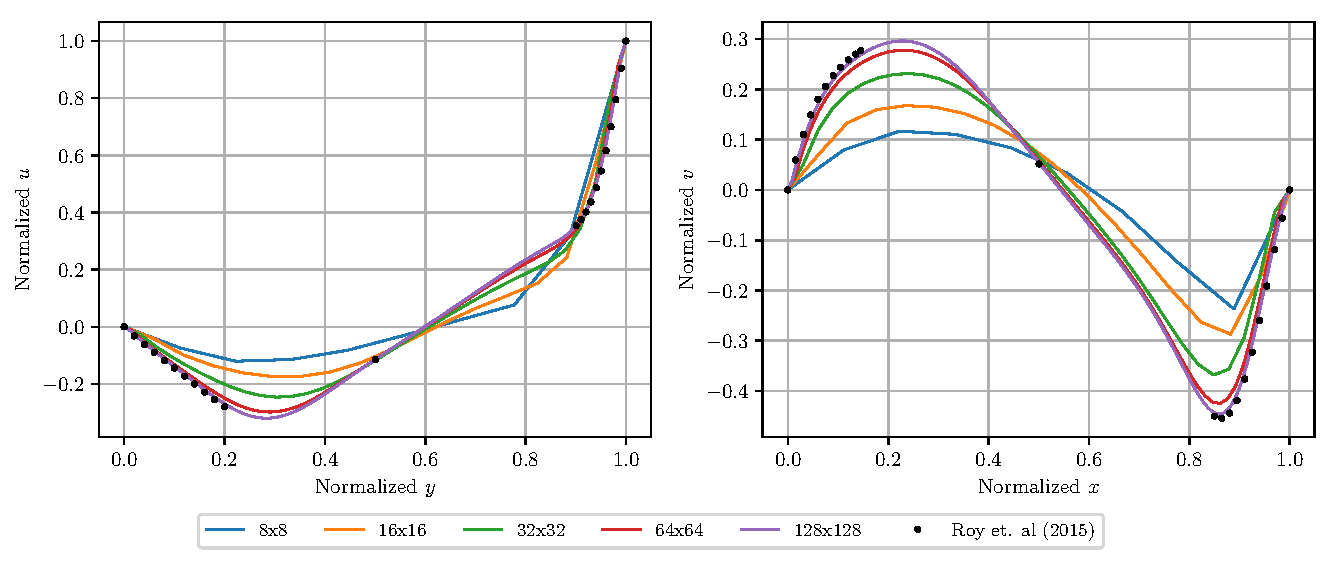
\includegraphics[width=\linewidth]{../results/p2}
	\caption{Centerline $u$ and $v$-velocity fields with the top plate pulled right at a constant velocity.}
	\label{fig:p2}
\end{figure}

\section*{Code listing}

For the implementation, we have the following files:
\begin{itemize}
	\item \texttt{Makefile} -- Allows for compiling the c++ project with \texttt{make}.
	\item \texttt{hwk4.cpp} -- Contains the \texttt{main()} function that is required by C that runs the cases requested in this problem set.
	\item \texttt{Problem.h} -- Contains the header for the \texttt{Problem} class which is the main driver for a \texttt{Flow2D::Problem}.
	\item \texttt{Variable.h} -- Contains the \texttt{Flow2D::Variable} class, which is a storage container for a single variable (i.e., $u$).
	\item \texttt{Problem.cpp} -- Contains the \texttt{run()} functions that executes a \texttt{Problem}.
	\item \texttt{Problem\_coefficients.cpp} -- Contains the functions for solving coefficients in a \texttt{Problem}.
	\item \texttt{Problem\_corrections.cpp} -- Contains the functions for correcting solutions in a \texttt{Problem}.
	\item \texttt{Problem\_residuals.cpp} -- Contains the functions for computing residuals in a \texttt{Problem}.
	\item \texttt{Problem\_solvers.cpp} -- Contains the functions for sweeping and solving in a \texttt{Problem}.
	\item \texttt{Matrix.h} -- Contains the \texttt{Matrix} class which provides storage for a matrix with various standard matrix operations.
	\item \texttt{TriDiagonal.h} -- Contains the \texttt{TriDiagonal} class which provides storage for a tri-diagonal matrix including the TDMA solver found in the member function \texttt{solveTDMA()}.
	\item \texttt{Vector.h} -- Contains the \texttt{Vector} class for one-dimensional vector storage.
	\item \texttt{plots.py} - Produces the plots in this report.
\end{itemize}

\subsection*{Makefile}
\inputminted[fontsize=\scriptsize]{Makefile}{../Makefile}

\subsection*{hwk4.cpp}
\inputminted[fontsize=\scriptsize]{c++}{../hwk4.cpp}

\newpage
\subsection*{Problem.h}
\inputminted[fontsize=\scriptsize]{c++}{../Problem.h}

\newpage
\subsection*{Variable.h}
\inputminted[fontsize=\scriptsize]{c++}{../Variable.h}

\newpage
\subsection*{Problem.cpp}
\inputminted[fontsize=\scriptsize]{c++}{../Problem.cpp}

\newpage
\subsection*{Problem\_coefficients.cpp}
\inputminted[fontsize=\scriptsize]{c++}{../Problem_coefficients.cpp}

\newpage
\subsection*{Problem\_corrections.cpp}
\inputminted[fontsize=\scriptsize]{c++}{../Problem_corrections.cpp}

\newpage
\subsection*{Problem\_residuals.cpp}
\inputminted[fontsize=\scriptsize]{c++}{../Problem_residuals.cpp}

\newpage
\subsection*{Problem\_solvers.cpp}
\inputminted[fontsize=\scriptsize]{c++}{../Problem_solvers.cpp}

\newpage
\subsection*{Matrix.h}
\inputminted[fontsize=\scriptsize]{c++}{../Matrix.h}

\newpage
\subsection*{TriDiagonal.h}
\inputminted[fontsize=\scriptsize]{c++}{../TriDiagonal.h}

\newpage
\subsection*{Vector.h}
\inputminted[fontsize=\scriptsize]{c++}{../Vector.h}

\newpage
\subsection*{plots.py}
\inputminted[fontsize=\scriptsize]{python}{../plots.py}

\end{document}
